
\documentclass[12pt]{article}

\usepackage{graphicx}
\graphicspath{ {./images/} }

\usepackage{epsfig}
\usepackage{amsmath,amsthm}
\usepackage{listings}


\newtheorem{lemma}{Lemma}
\newtheorem{theorem}{Theorem}


\usepackage{titlesec}
\titleformat{\section}
{\normalfont\Large\bfseries}{Question~\thesection:}{1em}{}

\newlength{\toppush}
\setlength{\toppush}{2\headheight}
\addtolength{\toppush}{\headsep}


\def\subjnum{Comp 170}
\def\subjname{Computation Theory}


\def\doheading#1#2#3{\vfill\eject\vspace*{-\toppush}%
  \vbox{\hbox to\textwidth{{\bf} \subjnum: \subjname \hfil Erli Cai}%
    \hbox to\textwidth{{\bf} Tufts University, Fall 2020 \hfil#3\strut}%
    \hrule}}


\newcommand{\htitle}[1]{\vspace*{1.25ex plus 1ex minus 0ex}%
\begin{center}
{\large\bf #1}
\end{center}} 



\begin{document}
\doheading{2}{title}{Homework 06}

\setlength\parindent{0pt}

\section{CFG $\rightarrow$PDA}

The PDA would be a 6 tuple $(Q,\Sigma,\Gamma, \delta,s,F)$
Q = {s,p,q}\\
$\Sigma = \{a,b\}$ \\ 
$\Gamma = {S,A,B,X}$\\
$s = s$\\
$F = {q}$\\
And $\delta$ is specified by the diagram below:\\
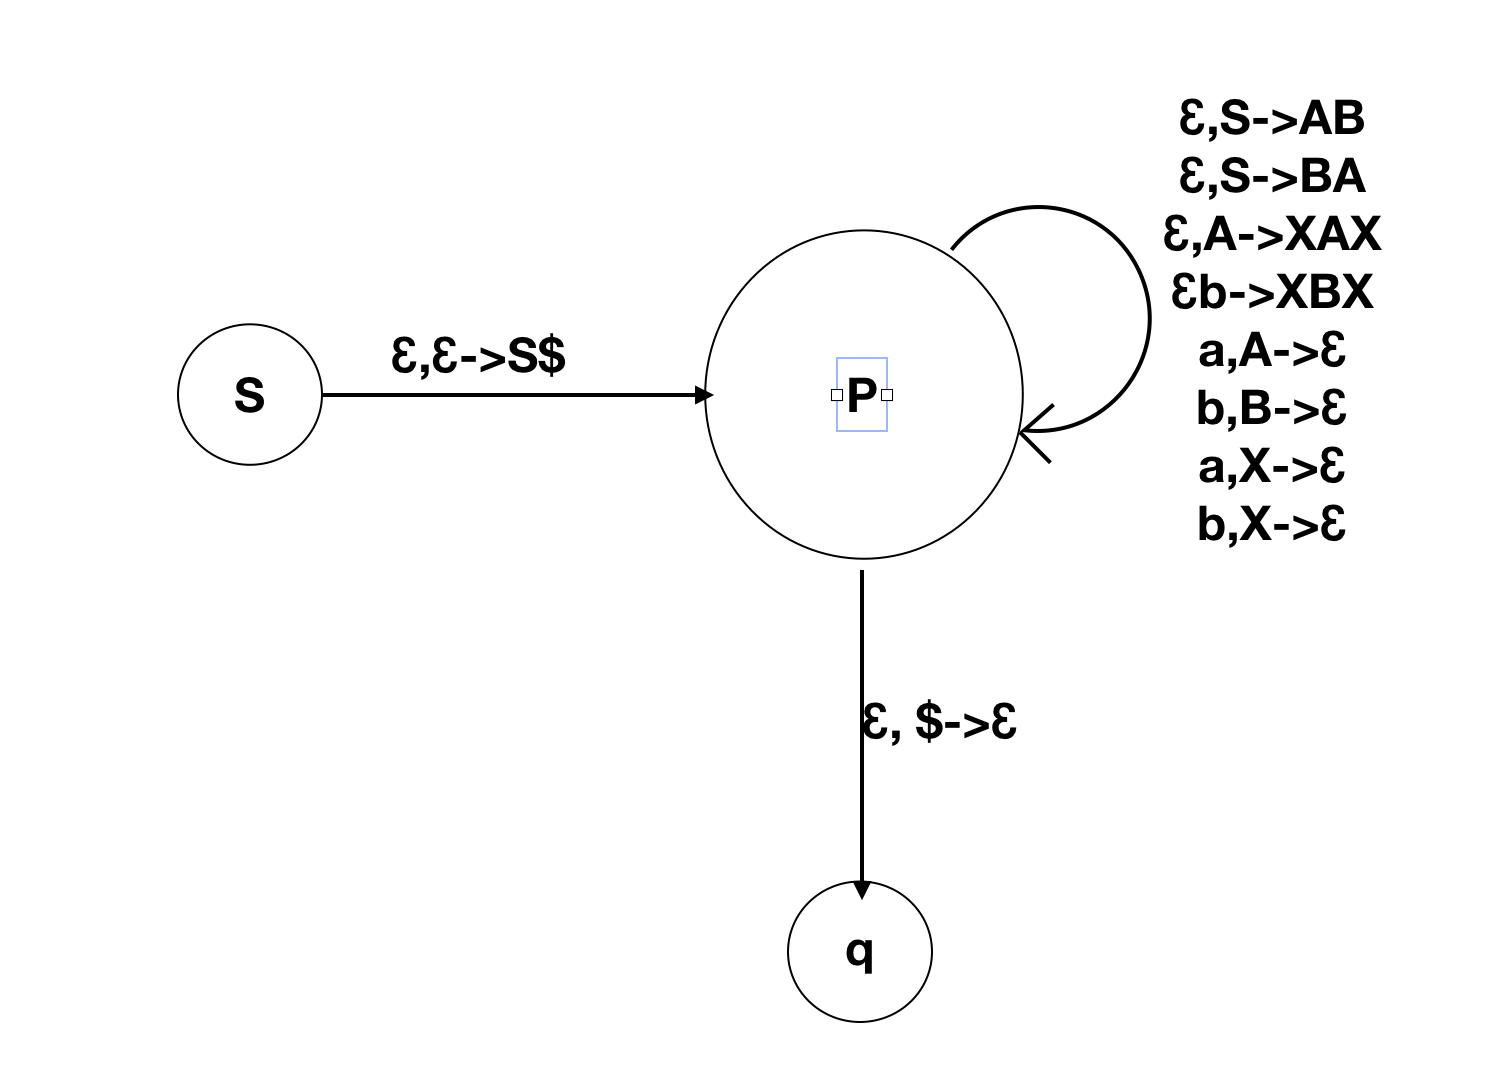
\includegraphics[scale = 0.5]{1}

\pagebreak
\section{Combining Machine Types}

$A/B = \{ w/wx\in A$ for some $x \in B   \}$

Assume we have a PDA $M_A$  = $(Q_A,\Sigma,\Gamma, \delta_A,s_A,F_A)$ that recognise A,\\
and a DFA $M_B$  = $(Q_B,\Sigma, \delta_B,s_B,F_B)$ that recognise B,\\
Then we can construct a PDA M = $(Q,\Sigma,\Gamma, \delta, s, F)$ that recognise A/B, where\\

$Q = Q_A \times Q_B \times (0,1)$\\
$\Gamma = \Gamma_A$\\

If $\delta_A(q_A,a,A)$ contains $(p_A, B)$, then in our new transition function,\\
$\delta((q_A,q_B,0),a,A)$ will contain $((p_A,q_B,0),B)$ and $((p_A,\delta(q_B,a),1),B)$\\
and $\delta((q_A,q_B,1),a,A)$ will contain $((p_A,\delta(q_B,a),1),B)$\\

$s = (s_A,s_B,0)$\\
$F = \{(q_a,q_b,q_c) | q_a \in F_A, q_b\in F_B\, q_c\in \{0,1\}\}$

\pagebreak
\section{Primal}

Consider a multi-tape Turing machine,\\
Tape one is the input string w with \$ on both end, the second tape starts with \$ a\$ \\ 

The Turing machine will do the following steps:\\
1. sweep left to right across both tapes one character at a time\\
2. If in step 1, the second tape reaches \$, then change the character in first tape to b. And let the pointer of the second tape goes back to the left most a.\\
3. If in step 1, the first tape reaches \$, check if the character on the left of the \$ is a or b\\
4. If in step 3, the character is b, then reject.\
5. If in step 3, the character is a, then add an a at the end of tape 2 and let the pointer of both tape goes back to the first character that is not \$, and sweep through both tapes at the same time.
6. If in step 5, the second tape reaches \$ before first tape, then sweep through first tape and change every character to a. Then goes back to step 1.
7, if in step 5, both tap reaches \$ at the same time, then reject








\end{document}


